\chapter{Conclusão}
\label{cap:conclusao}

Ao longo deste trabalho de conclusão de curso, realizamos atividades que passam
pelas principais áreas de conhecimento da Engenharia de Software, como a
gerência de projetos, a gerência de configuração de software,
o levantamento e a elaboração de requisitos, a análise e o \textit{design},
a implementação, e aqui incluimos a criação de testes automatizados,
a manutenção e a implantação de uma plataforma real de software livre, dentre
outras.
%
Nos preocupamos em contribuir, na prática, com a escrita de código~\footnote{%
Segue o link de alguns \textit{commits} realizado por nós durante a realização
deste trabalho: \\
\url{https://gitorious.org/noosfero/danielbucher-noosfero/commit/09c1af056d800c0f67632360734004b5c7090b7e}\\
\url{https://gitorious.org/noosfero/danielbucher-noosfero/commit/31298c57b1725da6fdc1b96744cecf232897d80f}}
, uma vez que, em nossa visão, esta é a principal missão de um Engenheiro de
Software.
%
Outra atividade que julgamos ser de fundamental importancia para a continuidade
deste trabalho, diz respeito ao repasse do conhecimento adquirido para uma
equipe de alunos do curso de Engenharia de Software, que trabalhou inicialmente
no Portal da FGA.

Esta experiência nos proporcionou a possibilidade de participar de um processo
distribuído de desenvolvimento de software com outras equipes espalhadas pelo
país e de fazer parte de uma comunidade de software livre.
%
Ao final deste trabalho, julgamos que a rede Comunidade.UnB está bem próxima
da capacidade de ser lançada oficialmente para a universidade, graças ao
apoio do CDTC, que viabilizou os contatos necessários para formalizar os
pedidos de uso, por exemplo, das bases de dados existentes nela, e graças
à comunidade do Noosfero que nos apoiou durante sua execução.

\begin{figure}[h!]
	\centering
	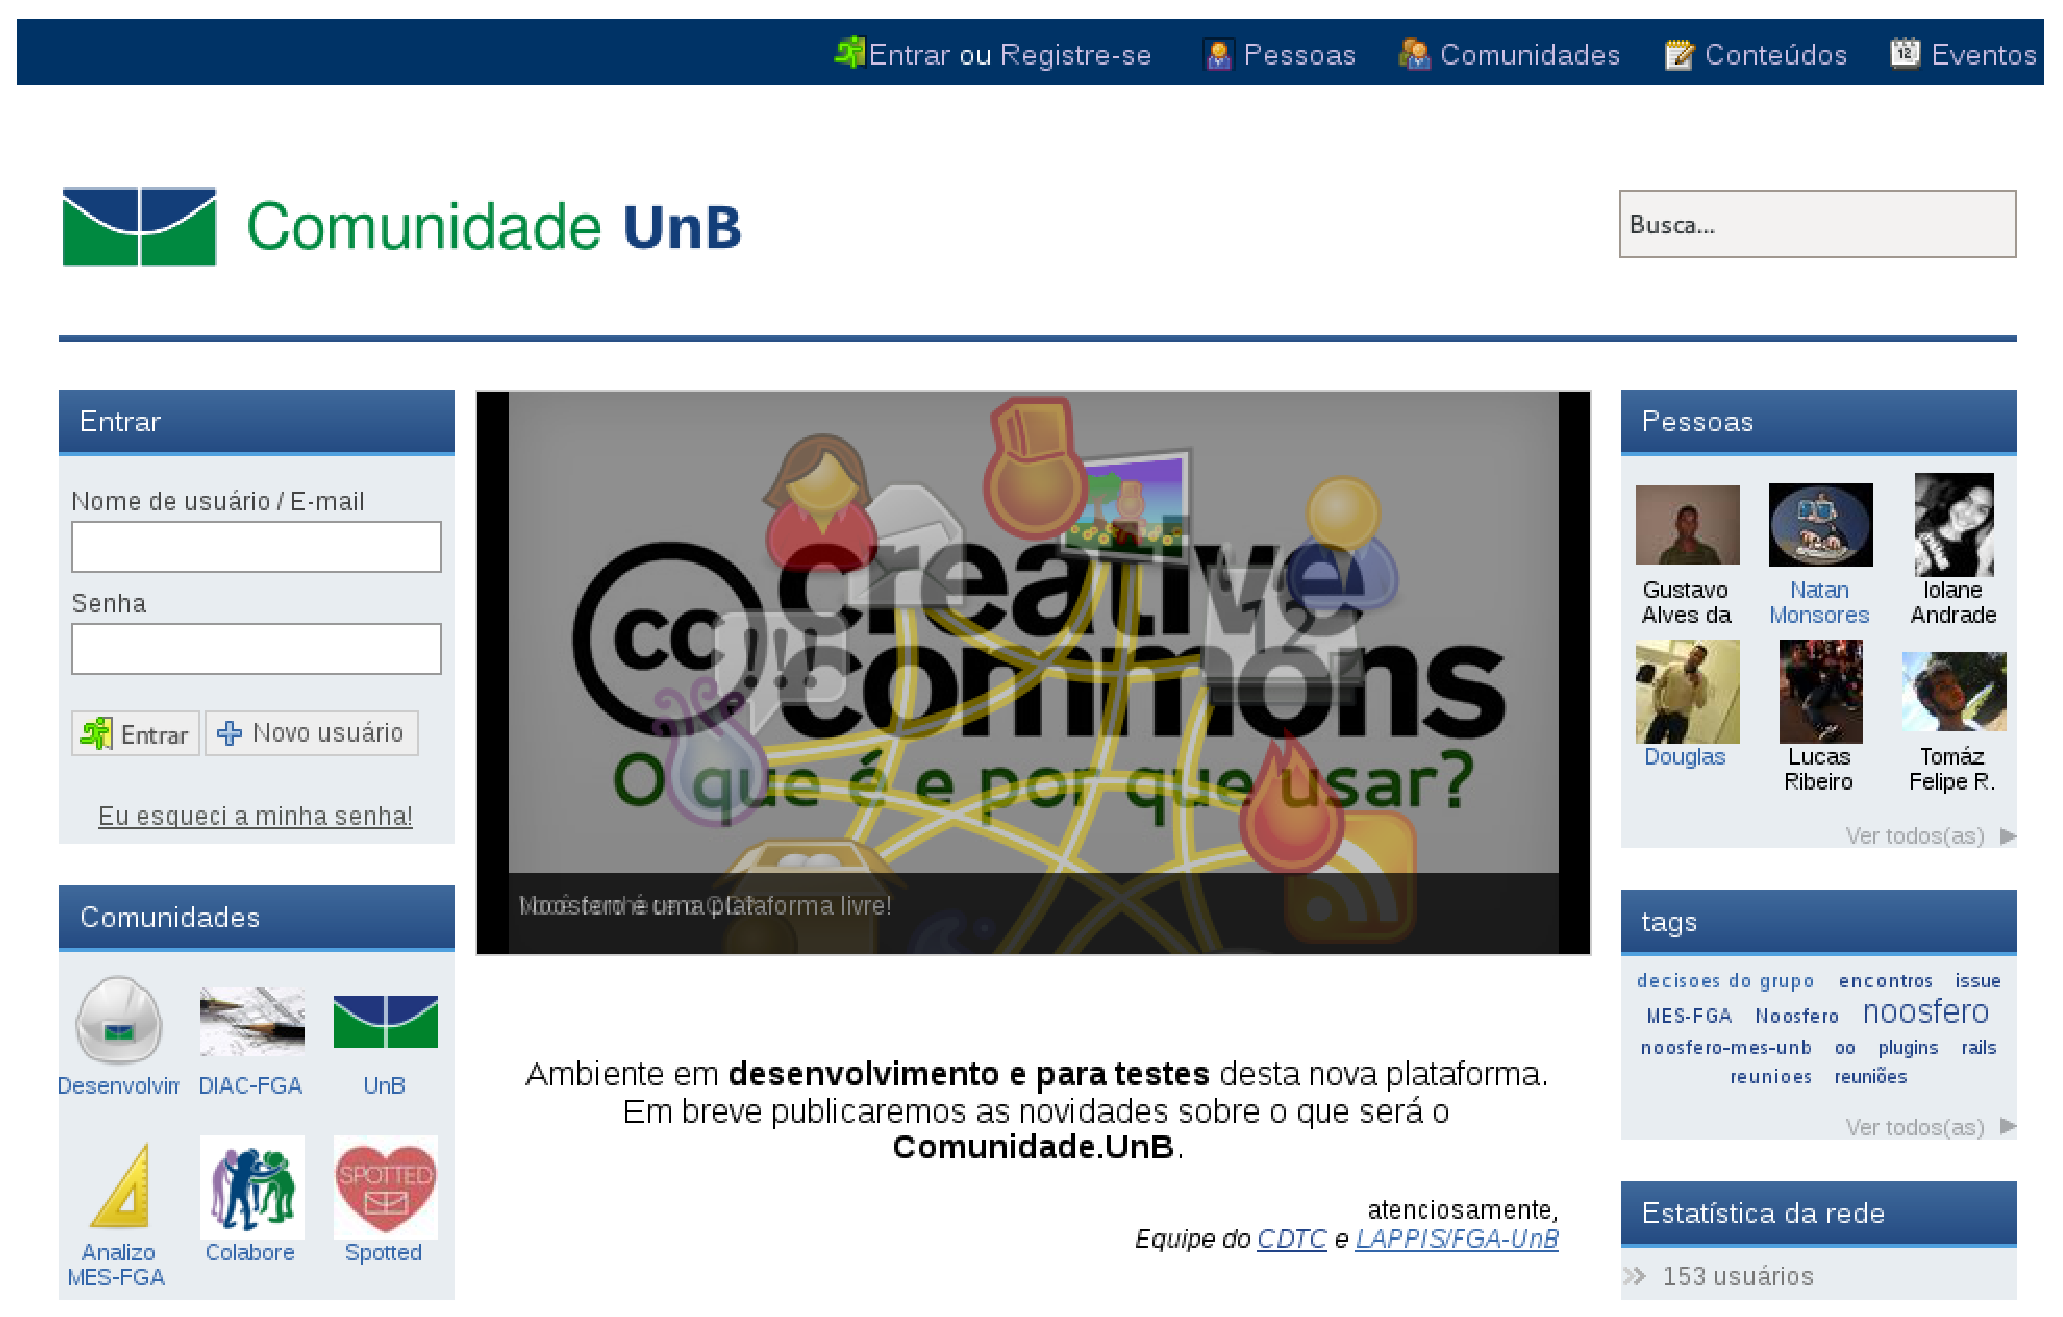
\includegraphics[keepaspectratio=true,scale=0.45]
	  {figuras/comunidade-unb.eps}
	\caption{Tela inicial da Comunidade.UnB}
	\label{homepage:comunidade.unb}
\end{figure}

A figura \ref{homepage:comunidade.unb} apresenta a página inicial do
Comunidade.UnB, ainda em ambiente de testes, que já consta com 153 usuários
e 14 comunidades.
%
Na próxima seção...

\begin{comment}
\section{Estado Atual}
%TODO Nao teremos estado atual e fim o que foi feito... ver onde colocaremos os proximos passos

O trabalho de implantação desta rede de colaboração conta com o apoio do \\ CDTC
~\footnote{\url{http://comunidade.cdtc.org.br/}}(Centro de Difusão de Tecnologia
e Conhecimento) que tem uma sede localizada no sub-solo do ICC no campus Darcy
Ribeiro. Esta parceria acelerou o processo de implantação de uma instância do
Noosfero (atualmente chamada de Comunidade.UnB) em um ambiente de
testes~\footnote{Disponível em \url{http://comunidade.unb.br}}, instalada em um
servidor do CDTC, que já está disponível para acesso externo. A Figura
\ref{comunidade-unb} apresenta a tela inicial da rede de colaboração da UnB
em seu ambiente de testes.

\begin{figure}[h]
	\centering
	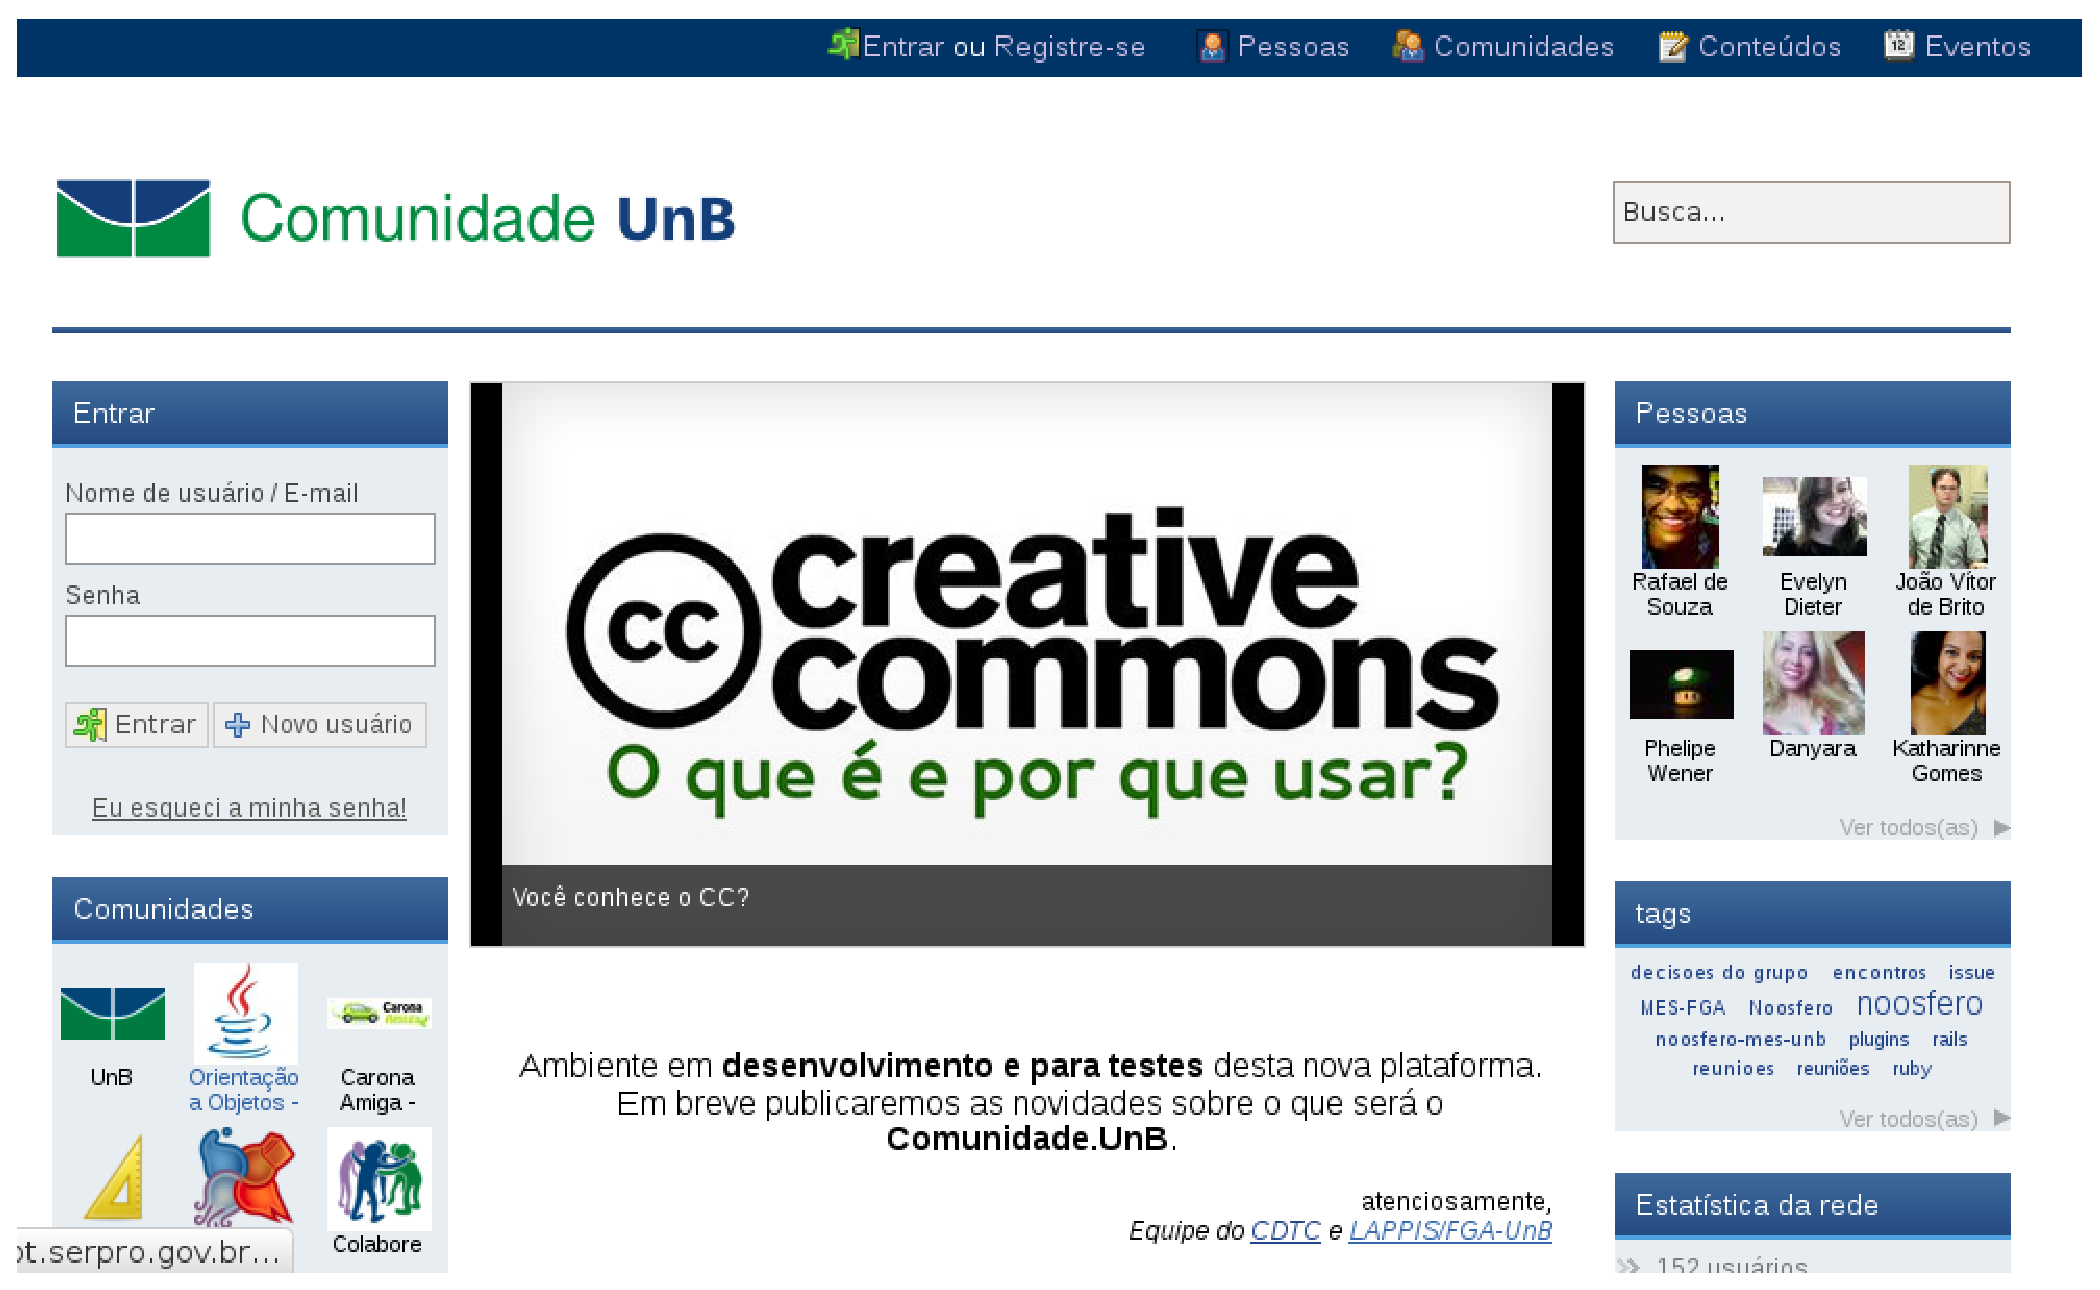
\includegraphics[keepaspectratio=true,scale=0.3]
	  {figuras/comunidade.unb.br.eps}
	\caption{Tela inicial da Comunidade.UnB}
	\label{comunidade-unb}
\end{figure}

O apoio institucional é fundamental para o funcionamento deste trabalho de forma
contínua uma vez que queremos que a Comunidade.UnB seja a rede de colaboração
oficial da Universidade. Portanto, pretendemos utilizar este trabalho como um
ponto de partida para formalizar uma proposta de criação de um projeto de
desenvolvimento e manutenção desta rede através da colaboração de alunos
bolsistas. Por exemplo, já foi submetida uma solicitação de bolsas para um projeto
de iniciação científica no edital do ProIC (Projeto de Iniciação científica)
aberto no primeiro semestre de 2013 pelo DPP (Decanato de Pesquisa e Pós-
Graduação) da UnB.

\end{comment}

\section{Trabalhos futuros}
\label{sec:future-works}

%TODO compra de certificado

\subsection{Federação}

A transição do Noosfero para uma rede social federada é essencial para a criação
de um ecosistema de redes de colaboração que comunicam entre si. A federação
consiste na habilidade de redes diferentes de conversarem entre si de forma que
um usuário da rede Comunidade.UnB poderia receber atualizações de uma comunidade
em outra rede baseada em Noosfero ou em qualquer outra ferramenta que implemente
o mesmo protocolo de federação, através de regras pré-acordadas
\cite{prodomou2010}.

Em princípio, a estrutura para redes federadas proposta para a plataforma Noosfero
consistia em um padrão aberto, chamado OStatus
~\footnote{\url{http://www.w3.org/community/ostatus/}}, que foi proposto
por Evan Prodomou para ser utilizado pelo StatusNet~\footnote{\url{
http://status.net/}}, um servidor  \textit{open-surce} para
\textit{microblogging} escrito em PHP.
%
O OStatus foi construído com base no padrõe para criação de \textit{feeds},
Atom~\footnote{\url{http://www.atomenabled.org/}} e no protocolo PuSH
~\footnote{\url{https://code.google.com/p/pubsubhubbub/}}(PubSubHubbub).
O funcionamento do OStatus pode ser resumido da seguinte forma:
os \textit{sites} produzem atualizações no formato de \textit{feeds} através
do padrão Atom e utilizam o protocolo PuSH para enviar estas atualizações
para outros \textit{sites} \cite{OStatusBasics}.
%
Posteriormente, OStatus passou a ser desenvolvido como um grupo de trabalho
da W3C e estava no caminho para se tornar um padrão oficial. 

No entanto, em dezembro de 2013, Prodomou declarou que estava desenvolvendo
um novo projeto chamado \textit{pump.io} quer iria substituir o StatusNEt
~\footnote{\url{http://status.net/2012/12/18/upcoming-changes-in-the-status
-net-service}} e que utilizará um novo protocolo para a federação chamado
Activity Streams~\footnote{\url{http://activitystrea.ms/}} baseado em JSON.
A adoção de um destes dois protocolos está sendo discutida pela comunidade do
Noosfero, mas já existe uma previsão para se começar a implementar a federação
para o mesmo, ainda em 2013. Parte deste trabalho consiste em colaborar com esta
implementação.

%-----------------------------------------------------------------------------%

\section{Próximas funcionalidades}

%------------------------------funcionalidade---------------------------------%
\subsection{Convite para participação de comunidades}

Esta funcionalidade prevê melhorias no sistema de convite para participar de
uma comunidade. Antes de sua implementação, os convites eram realizados
exclusivamente através de e-mail, seja entrando com o e-mail da pessoa
diretamente ou pesquisando na lista de contatos de um e-mail passado. Planejamos
esta funcionalidade para incluir uma interface através da qual um usuário
possa adicionar facilmente outros usuários da sua lista de amigos pesquisando
pelo nome, ou, caso deseje convidar um usuário do qual não seja amigo, ou alguém
que ainda não tenha cadastro na rede através do e-mail.

\subsubsection*{Histórias de usuário}

\begin{enumerate}

%--------------------------------história-------------------------------------%
\item Convidar usuários da rede

	\textbf{Para} facilitar a criação de convites para juntar-se a comunidade

	\textbf{Como} um membro de comunidade com permissão para convidar membros

	\textbf{Eu quero} convidar usuários através de uma interface que busque na lista
	de perfis de pessoas do ambiente e auto-complete conforme for digitando.

\subsubsection*{Cenários de uso}

	\begin{enumerate}

		\item Procurar um usuário cadastrado

		\textbf{Dado} que eu estou logado com meu usuário

		\textbf{E} meu usuário é administrador do Comunidade.UnB

		\textbf{E} o usuário `Zé' existe

		\textbf{E} o usuário `Zé' não é membro do Comunidade.UnB

		\textbf{E} eu estou na página de convidar amigos para o Comunidade.UnB

		\textbf{Quando} eu digitar `Zé' no campo de convidar novos amigos

		\textbf{Então} eu devo ver um \textit{token}\footnote{Neste contexto, um
		\textit{token} representa um objeto, no caso um perfil de usuário, que possua
		um nome que bata com o campo digitado.} representando o usuário `Zé'.

	\end{enumerate}


\end{enumerate}	

%TODO adicionar estudo sobre escalabilidade como trabalho futuro...


